%%%%%%%%%%%%%%%%%%%%%%%%%%%%%%%%%%%%%%%%%
% Lachaise Assignment
% LaTeX Template
% Version 1.0 (26/6/2018)
%
% This template originates from:
% http://www.LaTeXTemplates.com
%
% Authors:
% Marion Lachaise & François Févotte
% Vel (vel@LaTeXTemplates.com)
%
% License:
% CC BY-NC-SA 3.0 (http://creativecommons.org/licenses/by-nc-sa/3.0/)
% 
%%%%%%%%%%%%%%%%%%%%%%%%%%%%%%%%%%%%%%%%%

%----------------------------------------------------------------------------------------
%	PACKAGES AND OTHER DOCUMENT CONFIGURATIONS
%----------------------------------------------------------------------------------------

\documentclass{article}
\usepackage[portuguese]{babel}
\usepackage{enumerate}
\usepackage{graphicx}
\usepackage{hyperref}
\usepackage{float}
%%%%%%%%%%%%%%%%%%%%%%%%%%%%%%%%%%%%%%%%%
% Lachaise Assignment
% Structure Specification File
% Version 1.0 (26/6/2018)
%
% This template originates from:
% http://www.LaTeXTemplates.com
%
% Authors:
% Marion Lachaise & François Févotte
% Vel (vel@LaTeXTemplates.com)
%
% License:
% CC BY-NC-SA 3.0 (http://creativecommons.org/licenses/by-nc-sa/3.0/)
% 
%%%%%%%%%%%%%%%%%%%%%%%%%%%%%%%%%%%%%%%%%

%----------------------------------------------------------------------------------------
%	PACKAGES AND OTHER DOCUMENT CONFIGURATIONS
%----------------------------------------------------------------------------------------

\usepackage{amsmath,amsfonts,stmaryrd,amssymb} % Math packages

\usepackage{enumerate} % Custom item numbers for enumerations

\usepackage[ruled]{algorithm2e} % Algorithms

\usepackage[framemethod=tikz]{mdframed} % Allows defining custom boxed/framed environments

\usepackage{listings} % File listings, with syntax highlighting
\lstset{
	basicstyle=\ttfamily, % Typeset listings in monospace font
}

%----------------------------------------------------------------------------------------
%	DOCUMENT MARGINS
%----------------------------------------------------------------------------------------

\usepackage{geometry} % Required for adjusting page dimensions and margins

\geometry{
	paper=a4paper, % Paper size, change to letterpaper for US letter size
	top=2.5cm, % Top margin
	bottom=3cm, % Bottom margin
	left=2.5cm, % Left margin
	right=2.5cm, % Right margin
	headheight=14pt, % Header height
	footskip=1.5cm, % Space from the bottom margin to the baseline of the footer
	headsep=1.2cm, % Space from the top margin to the baseline of the header
	%showframe, % Uncomment to show how the type block is set on the page
}

%----------------------------------------------------------------------------------------
%	FONTS
%----------------------------------------------------------------------------------------

\usepackage[utf8]{inputenc} % Required for inputting international characters
\usepackage[T1]{fontenc} % Output font encoding for international characters

\usepackage{XCharter} % Use the XCharter fonts

%----------------------------------------------------------------------------------------
%	COMMAND LINE ENVIRONMENT
%----------------------------------------------------------------------------------------

% Usage:
% \begin{commandline}
%	\begin{verbatim}
%		$ ls
%		
%		Applications	Desktop	...
%	\end{verbatim}
% \end{commandline}

\mdfdefinestyle{commandline}{
	leftmargin=10pt,
	rightmargin=10pt,
	innerleftmargin=15pt,
	middlelinecolor=black!50!white,
	middlelinewidth=2pt,
	frametitlerule=false,
	backgroundcolor=black!5!white,
	frametitle={Command Line},
	frametitlefont={\normalfont\sffamily\color{white}\hspace{-1em}},
	frametitlebackgroundcolor=black!50!white,
	nobreak,
}

% Define a custom environment for command-line snapshots
\newenvironment{commandline}{
	\medskip
	\begin{mdframed}[style=commandline]
}{
	\end{mdframed}
	\medskip
}

%----------------------------------------------------------------------------------------
%	FILE CONTENTS ENVIRONMENT
%----------------------------------------------------------------------------------------

% Usage:
% \begin{file}[optional filename, defaults to "File"]
%	File contents, for example, with a listings environment
% \end{file}

\mdfdefinestyle{file}{
	innertopmargin=1.6\baselineskip,
	innerbottommargin=0.8\baselineskip,
	topline=false, bottomline=false,
	leftline=false, rightline=false,
	leftmargin=2cm,
	rightmargin=2cm,
	singleextra={%
		\draw[fill=black!10!white](P)++(0,-1.2em)rectangle(P-|O);
		\node[anchor=north west]
		at(P-|O){\ttfamily\mdfilename};
		%
		\def\l{3em}
		\draw(O-|P)++(-\l,0)--++(\l,\l)--(P)--(P-|O)--(O)--cycle;
		\draw(O-|P)++(-\l,0)--++(0,\l)--++(\l,0);
	},
	nobreak,
}

% Define a custom environment for file contents
\newenvironment{file}[1][File]{ % Set the default filename to "File"
	\medskip
	\newcommand{\mdfilename}{#1}
	\begin{mdframed}[style=file]
}{
	\end{mdframed}
	\medskip
}

%----------------------------------------------------------------------------------------
%	NUMBERED QUESTIONS ENVIRONMENT
%----------------------------------------------------------------------------------------

% Usage:
% \begin{question}[optional title]
%	Question contents
% \end{question}

\mdfdefinestyle{question}{
	innertopmargin=1.2\baselineskip,
	innerbottommargin=0.8\baselineskip,
	roundcorner=5pt,
	nobreak,
	singleextra={%
		\draw(P-|O)node[xshift=1em,anchor=west,fill=white,draw,rounded corners=5pt]{%
		Question \theQuestion\questionTitle};
	},
}

\newcounter{Question} % Stores the current question number that gets iterated with each new question

% Define a custom environment for numbered questions
\newenvironment{question}[1][\unskip]{
	\bigskip
	\stepcounter{Question}
	\newcommand{\questionTitle}{~#1}
	\begin{mdframed}[style=question]
}{
	\end{mdframed}
	\medskip
}

%----------------------------------------------------------------------------------------
%	WARNING TEXT ENVIRONMENT
%----------------------------------------------------------------------------------------

% Usage:
% \begin{warn}[optional title, defaults to "Warning:"]
%	Contents
% \end{warn}

\mdfdefinestyle{warning}{
	topline=false, bottomline=false,
	leftline=false, rightline=false,
	nobreak,
	singleextra={%
		\draw(P-|O)++(-0.5em,0)node(tmp1){};
		\draw(P-|O)++(0.5em,0)node(tmp2){};
		\fill[black,rotate around={45:(P-|O)}](tmp1)rectangle(tmp2);
		\node at(P-|O){\color{white}\scriptsize\bf !};
		\draw[very thick](P-|O)++(0,-1em)--(O);%--(O-|P);
	}
}

% Define a custom environment for warning text
\newenvironment{warn}[1][Warning:]{ % Set the default warning to "Warning:"
	\medskip
	\begin{mdframed}[style=warning]
		\noindent{\textbf{#1}}
}{
	\end{mdframed}
}

%----------------------------------------------------------------------------------------
%	INFORMATION ENVIRONMENT
%----------------------------------------------------------------------------------------

% Usage:
% \begin{info}[optional title, defaults to "Info:"]
% 	contents
% 	\end{info}

\mdfdefinestyle{info}{%
	topline=false, bottomline=false,
	leftline=false, rightline=false,
	nobreak,
	singleextra={%
		\fill[black](P-|O)circle[radius=0.4em];
		\node at(P-|O){\color{white}\scriptsize\bf i};
		\draw[very thick](P-|O)++(0,-0.8em)--(O);%--(O-|P);
	}
}

% Define a custom environment for information
\newenvironment{info}[1][Info:]{ % Set the default title to "Info:"
	\medskip
	\begin{mdframed}[style=info]
		\noindent{\textbf{#1}}
}{
	\end{mdframed}
}
 % Include the file specifying the document structure and custom commands
\usepackage{listings}

%----------------------------------------------------------------------------------------
%	ASSIGNMENT INFORMATION
%----------------------------------------------------------------------------------------

\title{EBD13 Gerência de Dados e Computação em Nuvem} % Title of the assignment

\author{Alexandre Miyazaki\\ \texttt{aksmiyazaki@gmail.com}} % Author name and email address

\date{Universidade Federal do Rio Grande do Sul} % University, school and/or department name(s) and a date

%----------------------------------------------------------------------------------------

\begin{document}

\maketitle % Print the title

\section{Introdução}
O objetivo do trabalho é analisar o Dataset do ENEM, assim como foi realizado o trabalho de EBD09. Todavia, agora usaremos Python e PySpark, fazendo o deploy de todo o ambiente na Google Cloud.

O objetivo é analisar o Dataset, além de comparar as facilidades e dificuldades de utilizar Python e R. Além disso, se houver tempo hábil, irei realizar também uma análise de desempenho simplificada, para determinar um mínimo local de arquitetura (número de workers) para executar as análises.


\subsection{Objetivo do Trabaho}

\subsection{Organização do Texto}

\newpage
\section{Dados}

Os dados utilizados foram os mesmos do trabalho de EBD09. Não irei entrar em detalhes de quantas \emph{features} existem nele, vamos fazer uma avaliação a medida que formos avançando na avaliação exploratória. Algumas características dos dados podem ser observadas na Tabela \ref{tab:data_data}.

\begin{table}[H]
\centering
\begin{tabular}{|c|c|c|c|}
\hline
Tamanho & Formato & Número de Features &  Número de Observações \\ \hline \hline
5.554 MB & CSV & 166 & 8.627.367 \\ \hline
\end{tabular}
\caption{Descrição dos Dados.}
\label{tab:data_data}
\end{table}

Para realizar todas as tarefas, foi submetido o dataset para o HDFS. O caminho completo do arquivo foi obtido navegando pelo sistema, conforme mostra a Figura \ref{fig:data_on_hdfs}.

\begin{figure}[H]
  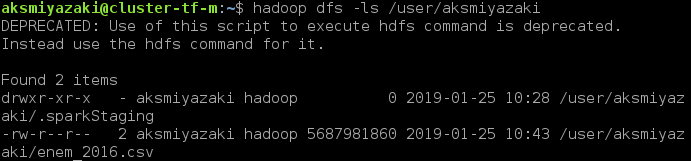
\includegraphics[width=\linewidth]{img/file_hdfs.png}
  \caption{Arquivos no HDFS, identificado como \emph{enem\_2016.csv}.}
  \label{fig:data_on_hdfs}
\end{figure}

\newpage
\section{Infraestrutura e Deploy de Ambiente}

Como base da infraestrutura, utilizou-se a parte de \emph{Data Proc} do Google Cloud. Inicialmente, criou-se um cluster com 1 \emph{master} e 2 \emph{slaves} apenas para a realização de um deploy inicial de todo o ambiente. A configuração dessas máquinas não necessariamente é importante pois só iremos setar o ambiente e testá-lo.

\subsection{Deploy de Ambiente}

Para fazer a avaliação da arquitetura, foram realizados testes de deploy do ambiente (nunca havia feito a implantação do ambiente com Jupyter na \emph{Google Cloud}).Felizmente a implantação das aplicações necessárias precisa apenas de uma ação: colocar o script \emph{gs://dataproc-initialization-actions/jupyter/jupyter.sh} como ação de inicialização.

Com isso, o ambiente montado já vem com Hadoop, Spark, PySpark, Jupyter e Anaconda, todos configurados. O último vem com um problema de configuração que não permite que sejam instalados novos pacotes. Isso foi resolvido executando o comando abaixo. Após esse comando, foi possível instalar pacotes normalmente (embora eu tenha dúvidas se essa é a melhor abordagem para a solução).

\begin{lstlisting}[caption= {Solução de problema de Permissão.},captionpos=b]
sudo chown -R $USER /opt/conda
\end{lstlisting}

\subsection{Avaliação de Arquitetura Ideal}

Antes de começar a efetivamente fazer a análise dos dados, decidi por avaliar algumas opções de arquitetura e ver qual seria a melhor opção (visto que, no momento, não estou preocupado com custo, apenas com desempenho). As arquiteturas testadas podem ser visualizadas na tabela \ref{tab:arqs}. Importante salientar que todas as arquiteturas possuem apenas um nó Master, cuja configuração é sempre igual a dos Slaves (a salvo na configuração 4, onde ele possui 2vCPU, 7.5GB de memória e 50 GB SSD).

Houveram problemas de alocação de arquitetura, pois há restrições no plano free da \emph{Google Cloud}. Conseguimos montar um cluster com no máximo 8 vCPUs e com no máximo 100GB (somatório total) de SSD. Portanto, analisei o que era possível ser criado.

A avaliação foi realizada inicialmente, apenas carregando os dados, com o trecho de código abaixo. Para cada execução, foi reiniciado o Kernel Python.

\begin{lstlisting}[caption= {Carga de dados no Spark},captionpos=b, language=python]
start = time.time()

df = sqlContext.read.option("delimiter", ';')
.load('hdfs:///user/aksmiyazaki/enem_2016.csv', 
                      format='com.databricks.spark.csv', 
                      header='true', 
                      inferSchema='true')

end = time.time()
t = end - start
\end{lstlisting}


\begin{table}[H]
\centering
\begin{tabular}{|c|c|c|c|c|}
\hline
Identificador & Número de Slaves & vCPUs &  Memória & Disco \\ \hline \hline
1 & 2 & 2 & 7,5 GB & 200GB HD  \\ \hline
2 & 2 & 2 & 7.5 GB & 30GB SSD \\ \hline
3 & 3 & 2 & 7.5 GB & 20GB SSD  slaves. \\ \hline
4 & 6 & 1 (VCPUj) & 3.75 GB & 100GB HD   \\ \hline
\end{tabular}
\caption{Descrição de Arquiteturas testadas.}
\label{tab:arqs}
\end{table}

Após a carga, foi criada uma \emph{lazily evaluated view} (trecho de código abaixo). Essa tabela pode ser consultada com SparkSQL. 

\begin{lstlisting}[caption= {Criação da Tabela para Consulta},captionpos=b, language=python]
df.createOrReplaceTempView("table_enem2016")
\end{lstlisting}

Com a tabela criada, os dados foram consultados utilizando o código abaixo. Essa consulta foi usada pois é necessário passar por todo o volume de dados para calcular a média de uma coluna (pelo menos por toda a coluna). Como os dados são distribuídos, mesmo sendo uma consulta simples, é uma forma adequada de fazer a avaliação. É importante salientar que nesse ponto o Kernel não é mais reinicializado.

\begin{lstlisting}[caption= {Consulta Simplificada para Avaliação},captionpos=b, language=python]
start = time.time()

df2 = spark.sql("Select mean(NU_NOTA_CN) from table_enem2016")
df2.collect()\

end = time.time()
\end{lstlisting}

Os resultados da avaliação (média de tempos) podem ser visualizados na Tabela \ref{tab:mean_times}. Para maiores detalhes, consulte a Seção \ref{sect:eval_data}

\begin{table}[H]
\centering
\begin{tabular}{|c|c|c|}
\hline
Configuração & Carga de Dados (média) &  Execução de  Consulta Simples (média) \\ \hline 
\hline
1 & 184.79 &  57.83
\\ \hline
2 & 172.98 & 49.72
 \\ \hline
3 & 124.81
 &  40.24
 \\ \hline
4 & 100.57
 &  27.92
 \\ \hline
\end{tabular}
\caption{Tempos médios de execução, em \textbf{segundos}.}
\label{tab:mean_times}
\end{table}

Algumas considerações sobre a análise:

\begin{itemize}
    \item Esperava que a configuração 2 tivesse um ganho bem maior em relação a 1, pois estamos usando SSD. Não cheguei a aprofundar a análise do motivo desse comportamento;
    \item A configuração 4 foi aquela que performou melhor. Mesmo a configuração anterior sendo equivalente em número de cores e armazenamento em SSD, muito provavelmente o gargalo é leitura de disco e nesse caso, tendo os dados distribuídos em mais workers acabou sendo mais impactante;
    \item Possívelmente haveriam outras configurações melhores, se não tivéssemos limites de alocação.
\end{itemize}

Portanto, a arquitetura de número 4 é a mais performática em termos de processamento e é a que iremos utilizar no trabalho. Ela não é tão adequada para o processamento de grandes volumes de dados (em uma consulta simples, levando em torno de 27 segundos), mas é a melhor que conseguimos montar no ambiente disponibilizado. É importante salientar também que essa configuração pode não ser o melhor custo benefício (isso precisaria ser levado em consideração no mundo real).

A Figura \ref{fig:hdfs_data} mostra as estatísticas do master e de um dos datanodes (slaves) após a carga de dados. Pode-se notar que a arquitetura utilizada possui 6 slaves pela linha que reporta o número de Live datanodes.

\begin{figure}[H]
\centering
  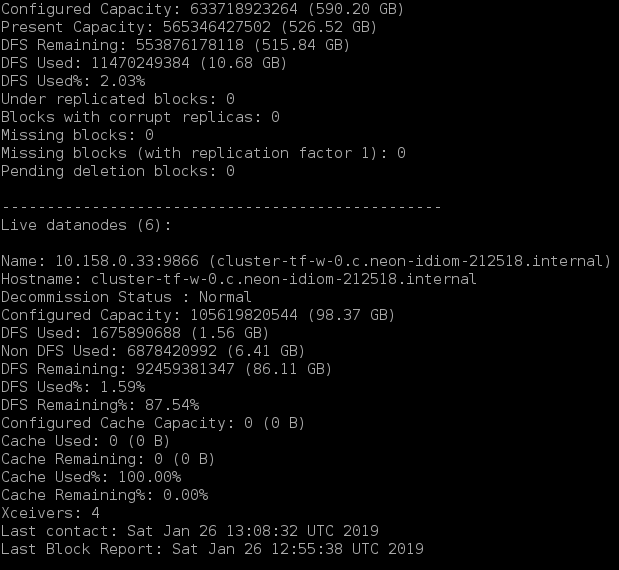
\includegraphics[width=0.6 \linewidth]{img/hdfs-occupation.png}
  \caption{Estatísticas do HDFS.}
  \label{fig:hdfs_data}
\end{figure}

Para ficar mais claro a arquitetura utilizada a Figura \ref{fig:arch} mostra sua representação. É importante notar que o Master possui configuração diferente dos Slaves.

\begin{figure}[H]
\centering
  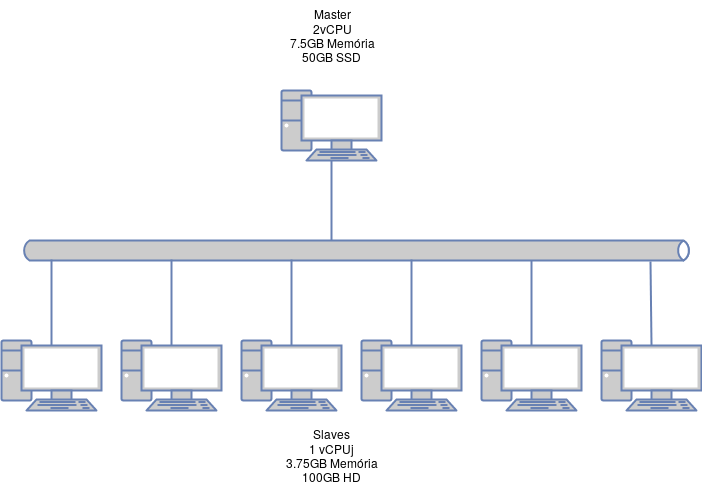
\includegraphics[width=0.8 \linewidth]{img/arch.png}
  \caption{Arquitetura utilizada no trabalho.}
  \label{fig:arch}
\end{figure}

\newpage
\section{Análise Exploratória dos Dados}

A análise dos dados tem como principal objetivo identificar \emph{Features} que tenham relação com as notas dos candidatos. Para isso, irei realizando inferências a medida que a análise avançar, exibindo os resultados obtidos.

A primeira intuição é avaliar se as regiões do País afetam as médias dos candidatos. Para isso, executou-se uma consulta , que calculava também a média total, gerando o gráfico da Figura \ref{fig:avg_uf}.

\begin{figure}[H]
\centering
  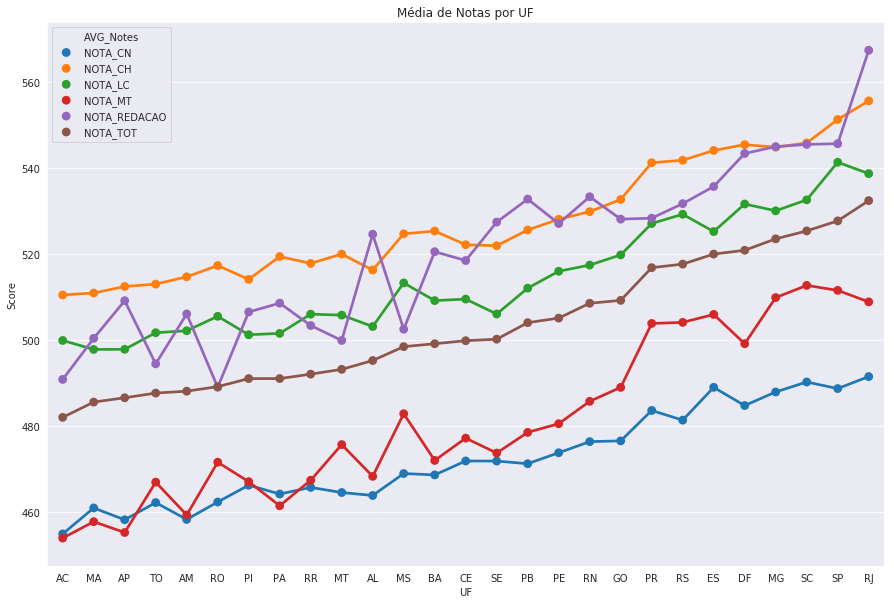
\includegraphics[width= 0.8 \linewidth]{img/mean_by_uf.png}
  \caption{Médias por UF.}
  \label{fig:fig_maq_criad}
\end{figure}

É visível a discrepância de notas da parte sudeste do país com o restante. Portanto, concluí-se que essa é uma \emph{Feature} bem significativa para inferir a nota do candidato.

Fazendo uma análise da idade relacionada a média total, podemos ver uma tendência decrescente nos dados a medida que a idade aumenta, na Figura \ref{fig:mean_by_age}. Analisando a correlação de Idade com a média total, temos um valor de -0.52, o que indica uma correlação negativa razoável (a medida que aumenta a idade, a média cai, o que confirma a análise visual).

\begin{figure}[H]
\centering
  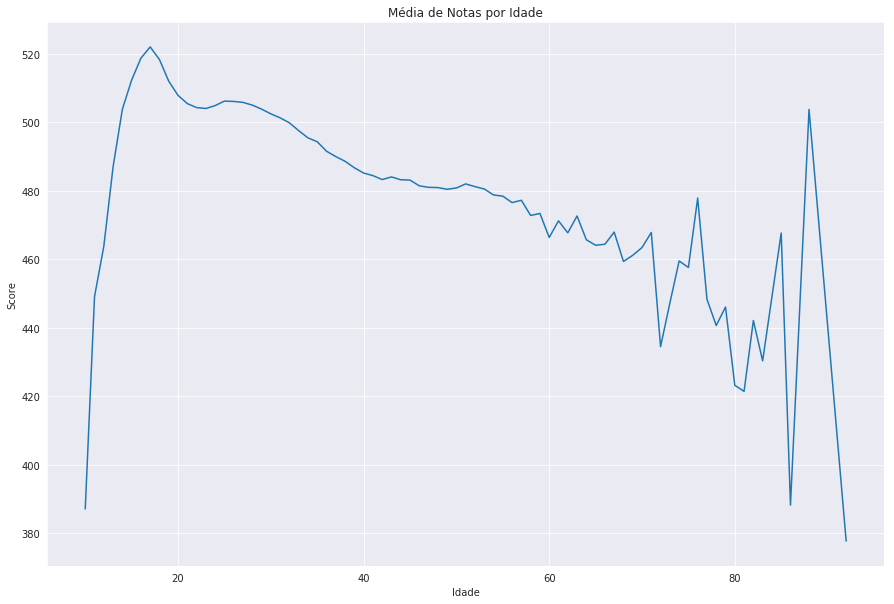
\includegraphics[width=0.8 \linewidth]{img/mean_by_age.png}
  \caption{Médias por Idade.}
  \label{fig:mean_by_age}
\end{figure}

Também foi realizada uma análise, verificando a renda familiar (informada na Feature Q006). A renda é representada por letras, onde A indica sem renda e Q indica mais de R\$ 17.600,00 (ordem crescente). Na Figura \ref{fig:mean_by_wage} é visível a tendência crescente da média total a medida que a renda aumenta. É possível ver grandes discrepâncias nas notas de Redação e Matemática. Com isso, concluí-se que essa é uma Feature que também tem relação com a performance dos candidatos.

\begin{figure}[H]
\centering
  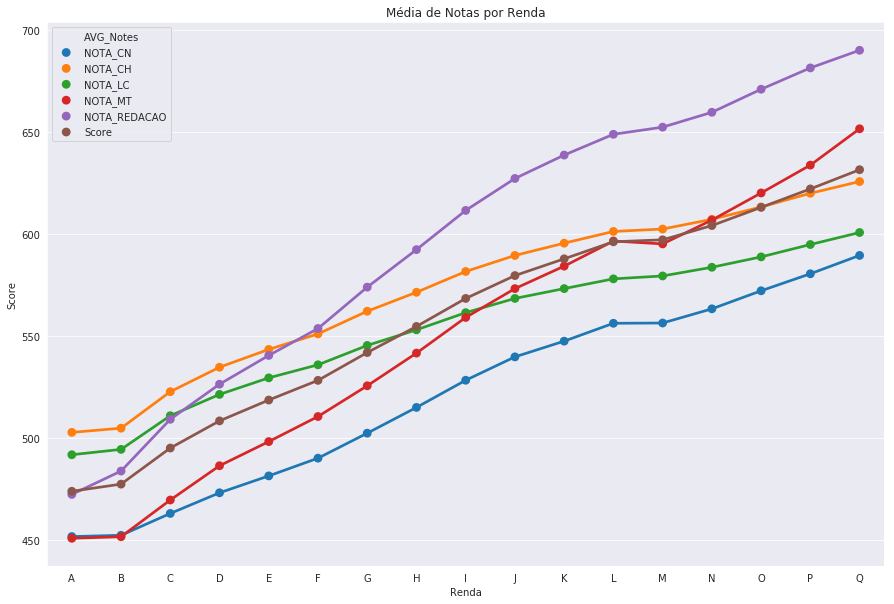
\includegraphics[width=0.8 \linewidth]{img/mean_by_wage.png}
  \caption{Médias por Faixa de Renda.}
  \label{fig:mean_by_wage}
\end{figure}

Também foi realizada uma análise por sexo, cujo resultado pode ser visualizado na Figura \ref{tab:mean_by_sex}. Notar que a diferença no Score total não foi significativa.

\begin{figure}[H]
\centering
  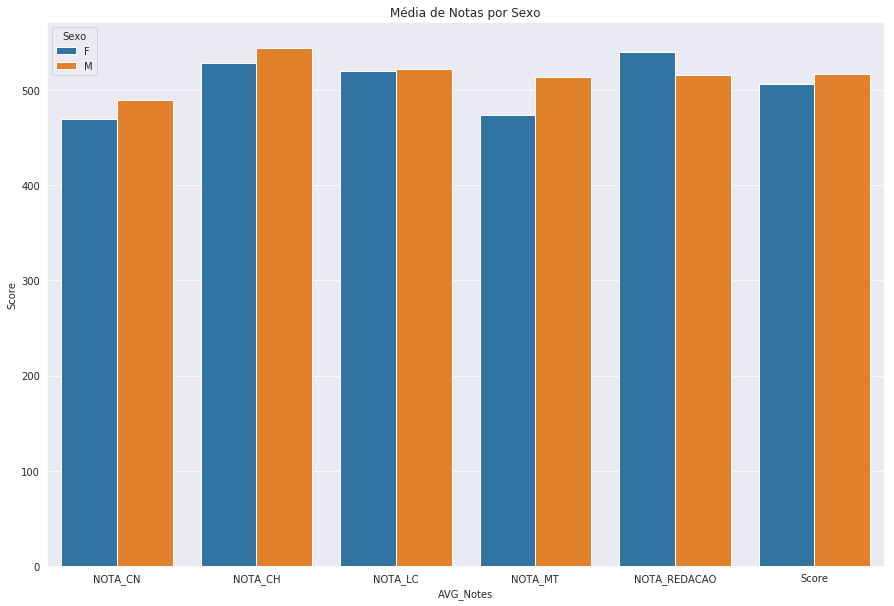
\includegraphics[width=0.8 \linewidth]{img/mean_by_sex.png}
  \caption{Médias por Sexo.}
  \label{fig:mean_by_sex}
\end{figure}

Analisando o estado civil dos candidatos, a Figura \ref{fig:mean_by_civil} mostra os resultados. Há uma clara relação deles com o score total (solteiros tiram notas maiores que os demais estados). É importante salientar que esses resultados podem estar correlacionados com Idade.

\begin{figure}[H]
\centering
  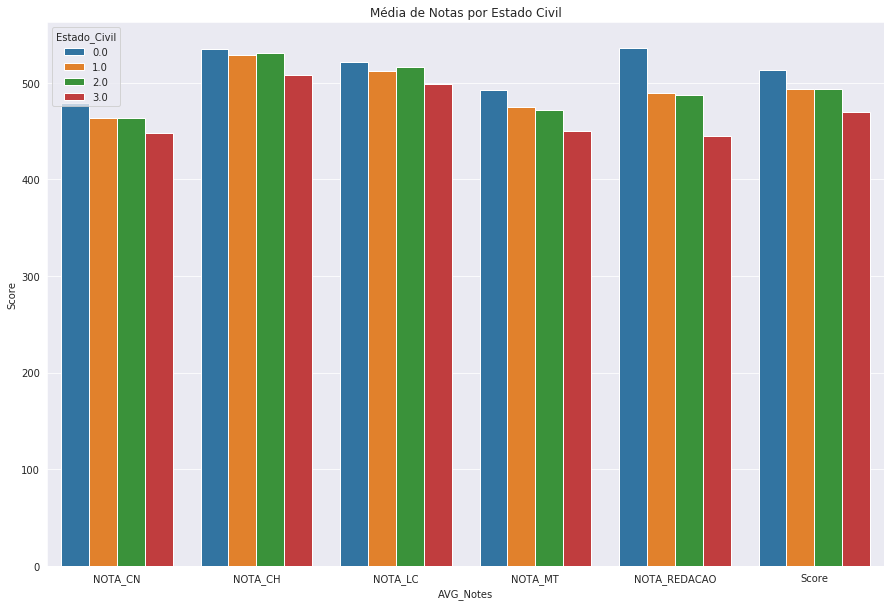
\includegraphics[width=0.8 \linewidth]{img/mean_by_civil.png}
  \caption{Médias por Estado Civil.}
  \label{fig:mean_by_sex}
\end{figure}

Ao analisar mais um campo, o de Raça, identificamos que há dois valores que não agregam tanta informação assim (Não Declarado e Não consta Informação). Há em torno de 165.000 registros com essas informações, todavia, nosso dataset possui mais de 8 milhões. Portanto, decidiu-se por avaliar assim mesmo, o resultado pode ser visualizado na Figura \ref{fig:mean_by_raca}. É possível notar que pessoas Brancas têm uma média superior as demais raças e, portanto, iremos considerar esse campo.

\begin{figure}[H]
\centering
  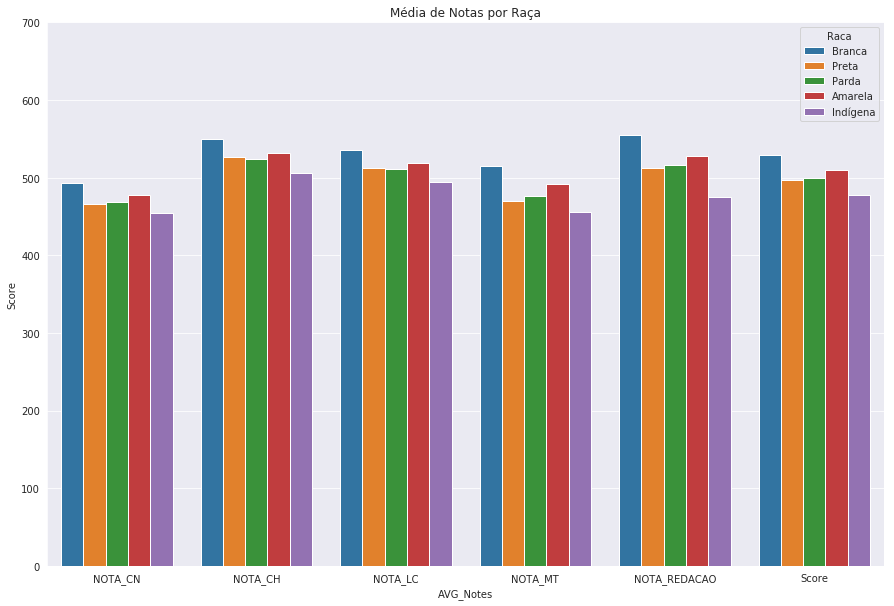
\includegraphics[width=0.8 \linewidth]{img/mean_by_raca.png}
  \caption{Médias por Raça declarada.}
  \label{fig:mean_by_raca}
\end{figure}





\newpage
\section*{Apêndice}
\label{sect:eval_data}
\subsection*{Execução de consultas por Arquitetura}

É importante notar que os identificadores citados nas Tabelas \ref{tab:times_load} e \ref{tab:query} se referem àqueles citados na Tabela \ref{tab:arqs}. A abordagem de avaliação foi bem simplificada, tendo em vista que fazer uma real análise de desempenho não faz parte do escopo do trabalho.

\begin{table}[H]
\centering
\begin{tabular}{|c|c|c|c|}
\hline
Identificador da Arquitetura & T1 & T2 & T3\\ \hline 
\hline
1 &  187.68613958358765 & 178.42478108406067 & 188.2514045238495\\ \hline
2 & 172.11613035202026 & 172.5200114250183 & 174.2983114719391 \\ \hline
3 & 127.42551612854
 & 121.673460960388
& 125.33324432373
\\ \hline
4 & 106.646942853928
 & 97.2526772022247
& 97.7907633781433
\\ \hline
\end{tabular}
\caption{Tempos de Carga, em \textbf{segundos}.}
\label{tab:times_load}
\end{table}

\begin{table}[H]
\centering
\begin{tabular}{|c|c|c|c|}
\hline
Identificador da Arquitetura & T1 & T2 & T3\\ \hline 
\hline
1 & 63.009117603302 & 61.09515404701233 & 49.37240242958069\\ \hline
2 & 58.08870315551758 & 46.74635648727417 & 44.3299551010132
\\ \hline
3 & 43.8593015670776
 & 44.337733745575
& 32.537876367569
\\ \hline
4 & 34.5449047088623
 & 24.7415041923523
& 24.4780607223511
\\ \hline
\end{tabular}
\caption{Tempos de Consulta, em \textbf{segundos}.}
\label{tab:query}
\end{table}



\end{document}

\begin{figure}[H]
  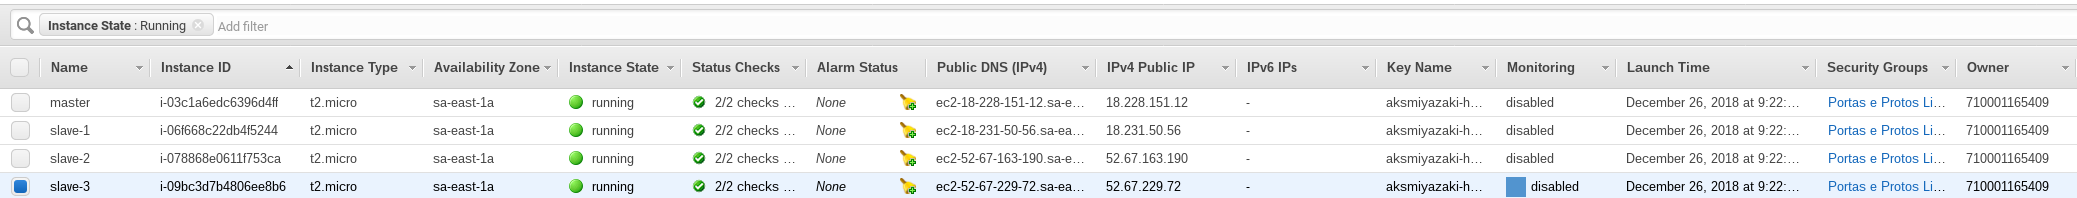
\includegraphics[width=\linewidth]{img/machines_created.png}
  \caption{Máquinas criadas na \emph{cloud}.}
  \label{fig:fig_maq_criad}
\end{figure}

